\documentclass{article}
\usepackage[utf8]{inputenc}
\usepackage[letterpaper,top=1.5cm,bottom=1.5cm,left=3cm,right=3cm,marginparwidth=1.75cm]{geometry}
\usepackage{natbib}
\usepackage{graphicx}
\usepackage{tikz}
\usepackage{amsmath, amsthm, amssymb, amsfonts}
\usepackage{titlesec}
\usepackage{pdflscape}
\usepackage{makecell}
\usepackage{xcolor,colortbl}
\usetikzlibrary{automata,positioning}
\usetikzlibrary{arrows}
\usepackage{inconsolata}
\usepackage{chessboard}
\storechessboardstyle{5x5}{maxfield=e5, labelbottomformat=}
\usetikzlibrary{shapes}
\makeatletter
\@addtoreset{subsection}{section}
\makeatother
\def\thesection{Question \arabic{section}}
\def\thesubsection{\arabic{section}. \textit{\alph{subsection}}}
\def\thesubsubsection{\arabic{section}. \textit{\alph{subsection}}. \textit{\roman{subsubsection}}}

\title{Artificial Intelligence\\Homework no. 3}
\author{Alireza Rostami\\Student Number: 9832090}
\date{}
\begin{document}
    \maketitle
    \begin{center}
        Find the \LaTeX \ code of this masterpiece at my Github @ github.com/WellOfSorrows.
    \end{center}
   \section{}
   \subsection{}
   \subsubsection{}
   We would get:
    \begin{center}
    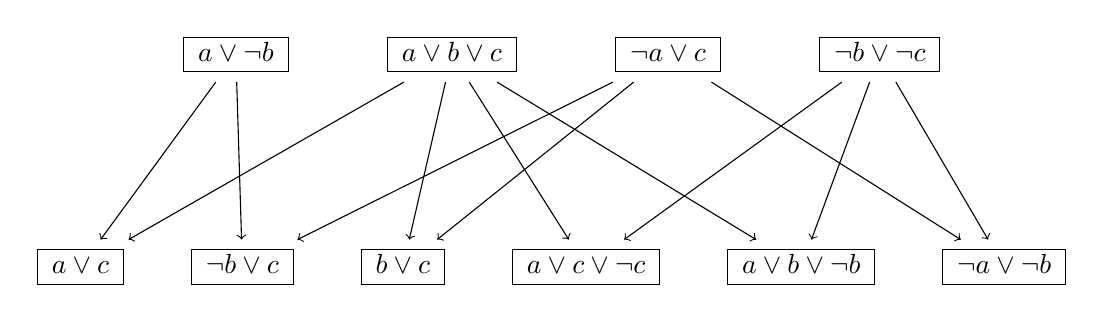
\begin{tikzpicture}
    \node (C1) at (0,0) {
        $\begin{array}{|c|}
            \hline
            a \vee \neg b \\
            \hline
        \end{array}$
    };
    \node[right=10mm of C1] (C2) {
        $\begin{array}{|c|}
            \hline
            a \vee b \vee c \\
            \hline
        \end{array}$
    };
    \node[right=10mm of C2] (C3) {
        $\begin{array}{|c|}
            \hline
            \neg a \vee c \\
            \hline
        \end{array}$
    };
    \node[right=10mm of C3] (C4) {
        $\begin{array}{|c|}
            \hline
            \neg b \vee \neg c \\
            \hline
        \end{array}$
    };

    \node[below left=20mm and 5mm of C1] (nC1) {
        $\begin{array}{|c|}
            \hline
            a \vee c \\
            \hline
        \end{array}$
    };
    \node[right=6mm of nC1] (nC2) {
        $\begin{array}{|c|}
            \hline
            \neg b \vee c \\
            \hline
        \end{array}$
    };
    \node[right=6mm of nC2] (nC3) {
        $\begin{array}{|c|}
            \hline
            b \vee c \\
            \hline
        \end{array}$
    };   
    \node[right=6mm of nC3] (nC4) {
        $\begin{array}{|c|}
            \hline
            a \vee c \vee \neg c \\
            \hline
        \end{array}$
    };
    \node[right=6mm of nC4] (nC5) {
        $\begin{array}{|c|}
            \hline
             a \vee b \vee \neg b \\
            \hline
        \end{array}$
    };
    \node[right=6mm of nC5] (nC6) {
        $\begin{array}{|c|}
            \hline
            \neg a \vee \neg b \\
            \hline
        \end{array}$
    };
    \draw[->] (C1) edge (nC1);
    \draw[->] (C2) edge (nC1);
    \draw[->] (C1) edge (nC2);
    \draw[->] (C3) edge (nC2);
    \draw[->] (C2) edge (nC3);
    \draw[->] (C3) edge (nC3);
    \draw[->] (C2) edge (nC4);
    \draw[->] (C4) edge (nC4);
    \draw[->] (C2) edge (nC5);
    \draw[->] (C4) edge (nC5);
    \draw[->] (C3) edge (nC6);
    \draw[->] (C4) edge (nC6);
    \end{tikzpicture}
    \end{center}
    
    \subsubsection{}
    We would get:
    \begin{center}
    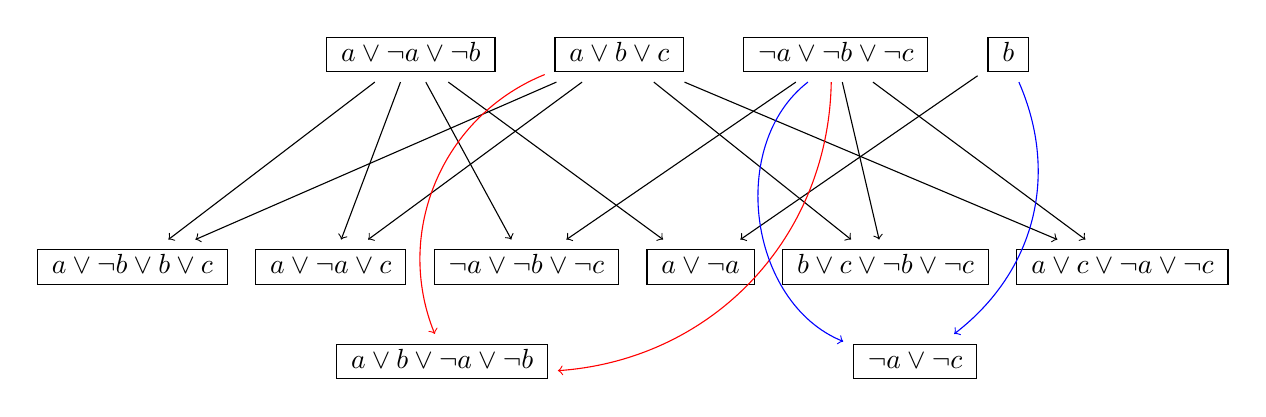
\begin{tikzpicture}
    \node (C1) at (0,0) {
        $\begin{array}{|c|}
            \hline
            a \vee \neg a \vee \neg b \\
            \hline
        \end{array}$
    };
    \node[right=5mm of C1] (C2) {
        $\begin{array}{|c|}
            \hline
            a \vee b \vee c \\
            \hline
        \end{array}$
    };
    \node[right=5mm of C2] (C3) {
        $\begin{array}{|c|}
            \hline
            \neg a \vee \neg b \vee \neg c \\
            \hline
        \end{array}$
    };
    \node[right=5mm of C3] (C4) {
        $\begin{array}{|c|}
            \hline
            b \\
            \hline
        \end{array}$
    };
    \node[below left=20mm and 10mm of C1] (nC1) {
        $\begin{array}{|c|}
            \hline
            a \vee \neg b \vee b \vee c \\
            \hline
        \end{array}$
    };
    \node[right=1mm of nC1] (nC2) {
        $\begin{array}{|c|}
            \hline
            a \vee \neg a \vee c \\
            \hline
        \end{array}$
    };
    \node[right=1mm of nC2] (nC3) {
        $\begin{array}{|c|}
            \hline
            \neg a \vee \neg b \vee \neg c \\
            \hline
        \end{array}$
    };
    \node[right=1mm of nC3] (nC4) {
        $\begin{array}{|c|}
            \hline
            a \vee \neg a \\
            \hline
        \end{array}$
    };
    \node[right=1mm of nC4] (nC5) {
        $\begin{array}{|c|}
            \hline
            b \vee c \vee \neg b \vee \neg c \\
            \hline
        \end{array}$
    };
    \node[right=1mm of nC5] (nC6) {
        $\begin{array}{|c|}
            \hline
            a \vee c \vee \neg a \vee \neg c \\
            \hline
        \end{array}$
    };
    \node[below left=5mm and 10mm of nC4] (nC7) {
        $\begin{array}{|c|}
            \hline
            a \vee b \vee \neg a \vee \neg b \\
            \hline
        \end{array}$
    };
    \node[below right=5mm and 10mm of nC4] (nC8) {
        $\begin{array}{|c|}
            \hline
            \neg a \vee \neg c \\
            \hline
        \end{array}$
    };
    \draw[->] (C1) edge (nC1);
    \draw[->] (C2) edge (nC1);
    \draw[->] (C1) edge (nC2);
    \draw[->] (C2) edge (nC2);
    \draw[->] (C1) edge (nC3);
    \draw[->] (C3) edge (nC3);
    \draw[->] (C1) edge (nC4);
    \draw[->] (C4) edge (nC4);
    \draw[->] (C2) edge (nC5);
    \draw[->] (C3) edge (nC5);
    \draw[->] (C2) edge (nC6);
    \draw[->] (C3) edge (nC6);
    \draw[->] (C2) edge [bend right = 45, red] (nC7);
    \draw[->] (C3) edge [bend left = 42.5, red] (nC7);
    \draw[->] (C3) edge [bend right = 60, blue] (nC8);
    \draw[->] (C4) edge [bend left = 38, blue] (nC8);
    \end{tikzpicture}
    \end{center}

    \newpage
   \subsection{}
   To write the CNF form of the first and the third sentence, we eliminate $\Rightarrow$.
   \begin{align*} \begin{split}
        &P(x) \rightarrow Q(x) \vee M(x) \\
        \text{is equivalent to  } \neg &P(x) \vee Q(x) \vee M(x)
    \end{split} \end{align*}
    \medskip
    \begin{align*} \begin{split}
        \neg &M(y) \rightarrow \neg (\neg P(x) \wedge R(x,y)) \\
        \text{is equivalent to  } \neg &M(y) \rightarrow P(x) \vee \neg R(x,y) \\
        \text{is equivalent to  } &M(y) \vee P(x) \vee \neg R(x,y) \\
    \end{split} \end{align*}
    \bigskip
    \\
    Thus, our CNF-normal \textit{KB} is:
    \begin{align*}
        &M(y) \vee P(x) \vee \neg R(x,y) \\
        \neg &P(x) \vee Q(x) \vee M(x) \\
        \neg &Q(x)\vee R(y,x) \vee \neg P(y) \\
        &R(\text{John}, \text{Pit}) \\
        \neg &R(\text{John}, \text{Mary}) \\
        &P(\text{Pit}) \\
        &Q(\text{Mary})
    \end{align*}
    To use resolution algorithm, we must show \textit{KB} $\wedge \neg M(x)$ leads to contradiction.\\
    \begin{landscape}
    \begin{center}
    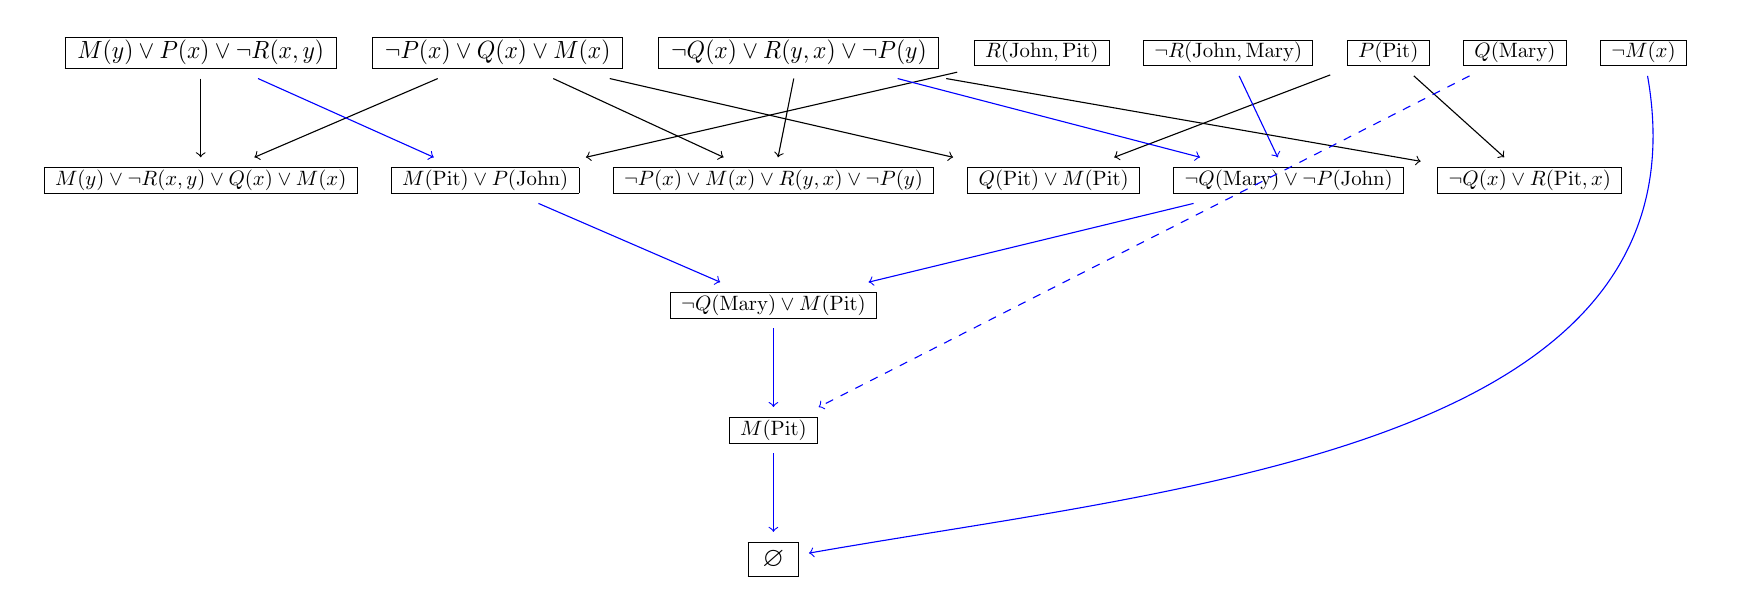
\begin{tikzpicture}
    % set up the nodes
    \node (C1) at (0,0) {
    \scalebox{0.85}[0.9]{    $\begin{array}{|c|}
            \hline
            M(y) \vee P(x) \vee \neg R(x,y) \\
            \hline
        \end{array}$
    }
    };
    \node[right=0.02mm of C1] (C2) {
     \scalebox{0.85}[0.9]{   $\begin{array}{|c|}
            \hline
            \neg P(x) \vee Q(x) \vee M(x) \\
            \hline
        \end{array}$
        }
    };
    \node[right=0.0002cm of C2] (C3) {
    \scalebox{0.85}[0.9]{    $\begin{array}{|c|}
            \hline
            \neg Q(x)\vee R(y,x) \vee \neg P(y) \\
            \hline
        \end{array}$
    }
    };
    \node[right=0.02mm of C3] (C4) {
    \scalebox{0.75}[0.75]{    $\begin{array}{|c|}
            \hline
            R(\text{John}, \text{Pit}) \\
            \hline
        \end{array}$
    }
    };
    \node[right=0.02mm of C4] (C5) {
    \scalebox{0.75}[0.75]{    $\begin{array}{|c|}
            \hline
            \neg R(\text{John}, \text{Mary}) \\
            \hline
        \end{array}$
    }
    };
    \node[right=0.02mm of C5] (C6) {
    \scalebox{0.75}[0.75]{
        $\begin{array}{|c|}
            \hline
            P(\text{Pit}) \\
            \hline
        \end{array}$
    }
    };
    \node[right=0.02mm of C6] (C7) {
    \scalebox{0.75}[0.75]{
        $\begin{array}{|c|}
            \hline
            Q(\text{Mary}) \\
            \hline
        \end{array}$
    }
    };
    \node[right=0.02mm of C7] (C8) {
    \scalebox{0.75}[0.75]{
        $\begin{array}{|c|}
            \hline
            \neg M(x) \\
            \hline
        \end{array}$
    }
    };
    \node[below=10mm of C1] (nC1)  {
    \scalebox{0.75}[0.75]{
        $\begin{array}{|c|}
            \hline
            M(y) \vee \neg R(x,y) \vee Q(x) \vee M(x)   \\
            \hline
        \end{array}$
    }
    };
    %\node[right=0.2mm of nC1] (nC2)  {
    %\scalebox{0.75}[0.75]{
    %    $\begin{array}{|c|}
    %        \hline
    %        M(y) \vee P(x) \vee \neg Q(x) \vee \neg P(y)   \\
    %        \hline
     %   \end{array}$
    %}
    %};
    \node[right=0.0002mm of nC1] (nC3)  {
    \scalebox{0.75}[0.75]{
        $\begin{array}{|c|}
            \hline
            M(\text{Pit}) \vee P(\text{John}) \\
            \hline
        \end{array}$
    }
    };
    \node[right=0.0002mm of nC3] (nC4)  {
    \scalebox{0.75}[0.75]{
        $\begin{array}{|c|}
            \hline
            \neg P(x) \vee M(x) \vee R(y,x) \vee \neg P(y) \\
            \hline
        \end{array}$
    }
    };
    \node[right=0.0002mm of nC4] (nC5)  {
    \scalebox{0.75}[0.75]{
        $\begin{array}{|c|}
            \hline
            Q(\text{Pit}) \vee M(\text{Pit}) \\
            \hline
        \end{array}$
    }
    };
    \node[right=0.0002mm of nC5] (nC6)  {
    \scalebox{0.75}[0.75]{
        $\begin{array}{|c|}
            \hline
            \neg Q(\text{Mary}) \vee \neg P(\text{John})  \\
            \hline
        \end{array}$
    }
    };
    \node[right=0.0002mm of nC6] (nC7)  {
    \scalebox{0.75}[0.75]{
        $\begin{array}{|c|}
            \hline
            \neg Q(x) \vee R(\text{Pit}, x)  \\
            \hline
        \end{array}$
    }
    };
    \node[below=10mm of nC4] (nnC1)  {
    \scalebox{0.75}[0.75]{
        $\begin{array}{|c|}
            \hline
            \neg Q(\text{Mary}) \vee M(\text{Pit})  \\
            \hline
        \end{array}$
    }
    };
    \node[below=10mm of nnC1] (nnnC1)  {
    \scalebox{0.75}[0.75]{
        $\begin{array}{|c|}
            \hline
            M(\text{Pit})  \\
            \hline
        \end{array}$
    }
    };
    \node[below=10mm of nnnC1] (nnnnC1)  {
        $\begin{array}{|c|}
            \hline
            \varnothing  \\
            \hline
        \end{array}$
    };
    % draw arrows and text between them
    \draw[->] (C1) edge (nC1);
    \draw[->] (C2) edge (nC1);
    \draw[->] (C1) edge [color=blue] (nC3);
    \draw[->] (C4) edge (nC3);
    \draw[->] (C2) edge (nC4);
    \draw[->] (C3) edge (nC4);
    \draw[->] (C2) edge (nC5);
    \draw[->] (C6) edge (nC5);
    \draw[->] (C3) edge [color=blue] (nC6);
    \draw[->] (C5) edge [color=blue] (nC6);
    \draw[->] (C3) edge (nC7);
    \draw[->] (C6) edge (nC7);
    \draw[->] (nC3) edge [color=blue] (nnC1);
    \draw[->] (nC6) edge [color=blue] (nnC1);
    \draw[->] (C7) edge [color=blue, dashed] (nnnC1);
    \draw[->] (nnC1) edge [color=blue] (nnnC1);
    \draw[->] (C8) edge [color=blue, out=-80, in=10] (nnnnC1);
    \draw[->] (nnnC1) edge [color=blue] (nnnnC1);
    \end{tikzpicture}
    \end{center}
    We reached contradiction; thus, the value of $M(x)$ is $ True $.
    \end{landscape}
    \section{}
    \subsection{}
    \subsubsection{}
    $$
        Mother(Mary, Charles) \Rightarrow \exists x \; Loves(x, Charles)
    $$
    \subsubsection{}
    $$
       \exists d \, \forall c \, \exists b \;\; Dog(d) \wedge Cat(c) \wedge Bird(b) \wedge Eat(c,b) \; \Rightarrow \; Hate(d,c)
    $$
    \subsection{}
    \subsubsection{}
    If a number is less than zero, then the cube of the number is also less than zero.
    \subsubsection{}
    There is some student that would teach every student who did not learn.
    \subsubsection{}
    Every student has at least two distinct friends. 
    \section{}
    \subsection{}
    One version of such assertion is:
    $$ KB = (\neg X_{1,2} \wedge X_{2,2} \wedge X_{2,1}) \vee ( X_{1,2} \wedge \neg X_{2,2} \wedge X_{2,1}) \vee ( X_{1,2} \wedge X_{2,2} \wedge \neg X_{2,1}) $$
    To translate the above DNF into CNF normal form, we can do the following. We know CNF normal form is equivalent to \textit{product-of-sums(POS)} form and DNF to \textit{sum-of-products(SOP)} form. Using these equivalences, we translate DNF form of our $ KB $ into SOP form:
    $$
        KB \equiv \overline{X_{1,2}} \cdot X_{2,2} \cdot X_{2,1} + {X_{1,2}} \cdot \overline{X_{2,2}} \cdot X_{2,1} + {X_{1,2}} \cdot X_{2,2} \cdot \overline{X_{2,1}}
    $$
    Using $X_{1, 2}$ as MSB, and considering we have three variables, we would get:
    $$
        KB \equiv \sum_{}^{} minterms(3,5,6) \equiv \prod_{}^{} Maxterms(0,1,2,4,7)
    $$
    Using the POS, we write the CNF form of our \textit{KB} as:
    \begin{align*}
    KB & \equiv 
        (\neg X_{1,2} \vee \neg X_{2,2} \vee \neg X_{2,1}) \\
        & \wedge 
        (\neg X_{1,2} \vee \neg X_{2,2} \vee X_{2,1}) \\ 
        & \wedge 
        (\neg X_{1,2} \vee X_{2,2} \vee \neg X_{2,1}) \\
        & \wedge 
        (X_{1,2} \vee \neg X_{2,2} \vee \neg X_{2,1}) \\
        & \wedge 
        (X_{1,2} \vee X_{2,2} \vee X_{2,1})
    \end{align*}
    \newpage
    \subsection{}
    The DNF form of such assertion is easy; since we have $k$ bombs in $n$ neighbors, thus, assuming neighbors of a each square are named $Y_1, Y_2, \dots, Y_n$, in each sentence $S_i$, $k$ variables are $True$ and other are $False$. Since we have $ t= \binom{n}{k} $ choices, we have $t$ sentences. Thus:
    $$ 
        \bigvee\limits_{i=1}^t S_i; \; \; \; \; \text{where} \; t = \binom{n}{k}
    $$
    To find the \textit{CNF} of \textit{KB}, we must find all the minterms of our \textit{KB}.\\
    To give an example, suppose $ S_{1} $ is the following:
    $$
        S_1 \equiv \overline{Y_n} \cdot \overline{Y_{n-1}} \; \dots \; \overline{Y_{k+1}} \cdot Y_{k} \; \dots \; Y_1
    $$
    The sentence $S_1$ corresponds to the following binary sequence:
    $$
        1 + 2 + \dots + 2^{k-1} = \sum_{i=0}^{k-1} 2^i = 2^{k} - 1
    $$
    Thus, $S_1$ corresponds to the minterm number $2^k - 1$. \\
    Doing such process for each $ S_i $, we find all the minterms. Suppose $m_i$ corresponds to $S_i$. Thus:
    $$
        KB \equiv \sum_{}^{} minterms(m_1, \dots, m_t) \equiv \prod_{}^{} Maxterms(M_1, \cdots, M_{2^n - t})
    $$
    Letting $M_i$ represent the CNF-normal sentence $S'_{i}$ and $t'$ as $2^n - t$, we arrive at:
    $$
        \bigwedge\limits_{i=1}^{t'} S'_i; \; \; \; \; \text{where} \; t' = 2^n - \binom{n}{k}
    $$
    %To simplify, since CNF is equivalent to POS, thus instead of writing $ Y_i $ if neighbor $ i $ contained a bomb, we write $ \neg Y_i $ if it contains one. Thus, for example $S'_i$ becomes:
    %$$
     %   S'_1 =  Y_n \wedge Y_{n-1} \wedge \; \dots \; \wedge Y_{n-k+1} \wedge \neg Y_{n-k} \wedge \; \dots \; \wedge \neg Y_1
    %$$
    \subsection{}
    For each cell we probe, the game gives a number $n$. We must construct a sentence with $\binom{n}{8}$ disjunct (supposing each cell has 8 neighbors, which is not always the case.) Conjoining all sentences together, we can use \textit{DPLL} in order to ascertain whether this sentence entails $X_{i,j}$ for any pair of $i, j$ we are concerned about.
    \subsection{}
    To modify our model in order for it to fit the global constraint, we construct a $\binom{M}{N}$ disjuncts, where each has $N$ variables. Since
    $$
        \binom{M}{N} = \frac{M}{M! (M-N)!}
    $$ 
    a Minesweeper game of 100 cells and 20 mines would contain $10^{39}$ disjuncts which is a bizarrely large number that no computer can process. To overcome such obstacle, we can append the global constraint to the DPLL itself. To achieve such goal, we can add $min$ and $max$ to DPLL algorithm, indicating the minimum and the maximum number of unassigned symbols that must be $True$ in the given model respectively. If there are no constraints, then we set $min = 0$ and $max = N$. Since Minesweeper is constrained, we cannot use such values. Thus, we set both $min = M$ and $max = M$ initially in the DPLL; and each time we call DPLL, we update $min$ and $max$ by subtracting one when assigning a $True$ value to a symbol. Within such process, if $min$ becomes less than the number of remaining symbols required to be $True$, since this is a contradiction, then we will exit the model immediately; or, if the $max$ becomes less than $0$, which is also a contradiction, we end the model. 
    \newpage
    \subsection{}
    There is no conclusions being invalidated via appending this ability to DPLL algorithm and taking the global constraint into consideration by using it.
    \subsection{}
    Consider the following configuration. 
    $$
    \begin{array}{|c|c|c|c|c|c|c|}
            \hline
            \cellcolor{black}{}&1&\cellcolor{black}{}&1&\cellcolor{black}{}&1&\cellcolor{black}{} \\\hline
        \end{array}
    $$
    There  are  two  possible  models: either mines are under every even-numbered black cell, or under every odd-numbered black cell. Making a probe at either end will entail whether cells at the far end are empty or contain mines.
    \section{}
    \subsection{}
    $$
        \exists d \; Parent(Joan, d) \wedge Female(d)
    $$
    \subsection{}
    \begin{align*}
        &\exists d \; Female(d) \wedge Parent(Joan, d) \wedge (\forall e \; (Female(e) \wedge e \neq d ) \Rightarrow \neg Parent(Joan, e)) \\
        \equiv \; &\exists^1 d \; Parent(Joan, d) \wedge Female(d)
    \end{align*}
    \subsection{}
    \begin{align*}
        \exists^1 d \; Female(d) \wedge Parent(Joan, d) \wedge (\forall e \; \neg Female(e) \Rightarrow \neg Parent(Joan, e))
    \end{align*}
    \subsection{}
    \begin{align*}
        \exists^1 c \; Parent(Joan, c) \wedge Parent(Kevin, c) 
    \end{align*}
    \subsection{}
    \begin{align*}
        \exists c \; Parent(Joan, c) \wedge Parent(Kevin, c) \wedge (\forall p \; (p \neq Kevin) \Rightarrow \nexists d  \; (Parent(Joan, d) \wedge Parent(p, d))
    \end{align*}
\end{document}
